
\documentclass[letterpaper,hide notes,xcolor={table,svgnames},pdftex,10pt]{beamer}
\def\showexamples{t}


%\usepackage[svgnames]{xcolor}

%% Demo talk
%\documentclass[letterpaper,notes=show]{beamer}

\usecolortheme{crane}
\setbeamertemplate{navigation symbols}{}

\usetheme{MyPittsburgh}
%\usetheme{Frankfurt}

%\usepackage{tipa}

\usepackage{hyperref}
\usepackage{graphicx,xspace}
\usepackage[normalem]{ulem}
\usepackage{multicol}
\usepackage{amsmath,amssymb,amsthm,graphicx,xspace}
\newcommand\SF[1]{$\bigstar$\footnote{SF: #1}}

\usepackage[default]{sourcesanspro}
\usepackage[T1]{fontenc}
\usepackage[scaled]{beramono}
\usepackage{tikzpagenodes}

\newcounter{tmpnumSlide}
\newcounter{tmpnumNote}


% old question code
%\newcommand\question[1]{{$\bigstar$ \small \onlySlide{2}{#1}}}
% \newcommand\nquestion[1]{\ifdefined \presentationonly \textcircled{?} \fi \note{\par{\Large \textbf{?}} #1}}
% \newcommand\nanswer[1]{\note{\par{\Large \textbf{A}} #1}}


 \newcommand\mnote[1]{%
   \addtocounter{tmpnumSlide}{1}
   \ifdefined\showcues {~\tiny\fbox{\arabic{tmpnumSlide}}}\fi
   \note{\setlength{\parskip}{1ex}\addtocounter{tmpnumNote}{1}\textbf{\Large \arabic{tmpnumNote}:} {#1\par}}}

\newcommand\mmnote[1]{\note{\setlength{\parskip}{1ex}#1\par}}

%\newcommand\mnote[2][]{\ifdefined\handoutwithnotes {~\tiny\fbox{#1}}\fi
% \note{\setlength{\parskip}{1ex}\textbf{\Large #1:} #2\par}}

%\newcommand\mnote[2][]{{\tiny\fbox{#1}} \note{\setlength{\parskip}{1ex}\textbf{\Large #1:} #2\par}}

\newcommand\mquestion[2]{{~\color{red}\fbox{?}}\note{\setlength{\parskip}{1ex}\par{\Large \textbf{?}} #1} \note{\setlength{\parskip}{1ex}\par{\Large \textbf{A}} #2\par}\ifdefined \presentationonly \pause \fi}

\newcommand\blackboard[1]{%
\ifdefined   \showblackboard
  {#1}
  \else {\begin{center} \fbox{\colorbox{blue!30}{%
         \begin{minipage}{.95\linewidth}%
           \hspace{\stretch{1}} Some space intentionally left blank; done at the blackboard.%
         \end{minipage}}}\end{center}}%
         \fi%
}



%\newcommand\q{\tikz \node[thick,color=black,shape=circle]{?};}
%\newcommand\q{\ifdefined \presentationonly \textcircled{?} \fi}

\usepackage{listings}
\lstset{basicstyle=\footnotesize\ttfamily,
	breaklines=true,
	aboveskip=15pt,
  	belowskip=15pt,
	frame=lines,
	numbers=left, basicstyle=\scriptsize, numberstyle=\tiny, stepnumber=0, numbersep=2pt
}

\usepackage{siunitx}
\newcommand\sius[1]{\num[group-separator = {,}]{#1}\si{\micro\second}}
\newcommand\sims[1]{\num[group-separator = {,}]{#1}\si{\milli\second}}
\newcommand\sins[1]{\num[group-separator = {,}]{#1}\si{\nano\second}}
\sisetup{group-separator = {,}, group-digits = true}

%% -------------------- tikz --------------------
\usepackage{tikz}
\usetikzlibrary{positioning}
\usetikzlibrary{arrows,backgrounds,automata,decorations.shapes,decorations.pathmorphing,decorations.markings,decorations.text,decorations.pathreplacing}

\tikzstyle{place}=[circle,draw=blue!50,fill=blue!20,thick, inner sep=0pt,minimum size=6mm]
\tikzstyle{transition}=[rectangle,draw=black!50,fill=black!20,thick, inner sep=0pt,minimum size=4mm]

\tikzstyle{block}=[rectangle,draw=black, thick, inner sep=5pt]
\tikzstyle{bullet}=[circle,draw=black, fill=black, thin, inner sep=2pt]

\tikzstyle{pre}=[<-,shorten <=1pt,>=stealth',semithick]
\tikzstyle{post}=[->,shorten >=1pt,>=stealth',semithick]
\tikzstyle{bi}=[<->,shorten >=1pt,shorten <=1pt, >=stealth',semithick]

\tikzstyle{mut}=[-,>=stealth',semithick]

\tikzstyle{treereset}=[dashed,->, shorten >=1pt,>=stealth',thin]

\usepackage{ifmtarg}
\usepackage{xifthen}
\makeatletter
% new counter to now which frame it is within the sequence
\newcounter{multiframecounter}
% initialize buffer for previously used frame title
\gdef\lastframetitle{\textit{undefined}}
% new environment for a multi-frame
\newenvironment{multiframe}[1][]{%
\ifthenelse{\isempty{#1}}{%
% if no frame title was set via optional parameter,
% only increase sequence counter by 1
\addtocounter{multiframecounter}{1}%
}{%
% new frame title has been provided, thus
% reset sequence counter to 1 and buffer frame title for later use
\setcounter{multiframecounter}{1}%
\gdef\lastframetitle{#1}%
}%
% start conventional frame environment and
% automatically set frame title followed by sequence counter
\begin{frame}%
\frametitle{\lastframetitle~{\normalfont(\arabic{multiframecounter})}}%
}{%
\end{frame}%
}
\makeatother

\makeatletter
\newdimen\tu@tmpa%
\newdimen\ydiffl%
\newdimen\xdiffl%
\newcommand\ydiff[2]{%
    \coordinate (tmpnamea) at (#1);%
    \coordinate (tmpnameb) at (#2);%
    \pgfextracty{\tu@tmpa}{\pgfpointanchor{tmpnamea}{center}}%
    \pgfextracty{\ydiffl}{\pgfpointanchor{tmpnameb}{center}}%
    \advance\ydiffl by -\tu@tmpa%
}
\newcommand\xdiff[2]{%
    \coordinate (tmpnamea) at (#1);%
    \coordinate (tmpnameb) at (#2);%
    \pgfextractx{\tu@tmpa}{\pgfpointanchor{tmpnamea}{center}}%
    \pgfextractx{\xdiffl}{\pgfpointanchor{tmpnameb}{center}}%
    \advance\xdiffl by -\tu@tmpa%
}
\makeatother
\newcommand{\copyrightbox}[3][r]{%
\begin{tikzpicture}%
\node[inner sep=0pt,minimum size=2em](ciimage){#2};
\usefont{OT1}{phv}{n}{n}\fontsize{4}{4}\selectfont
\ydiff{ciimage.south}{ciimage.north}
\xdiff{ciimage.west}{ciimage.east}
\ifthenelse{\equal{#1}{r}}{%
\node[inner sep=0pt,right=1ex of ciimage.south east,anchor=north west,rotate=90]%
{\raggedleft\color{black!50}\parbox{\the\ydiffl}{\raggedright{}#3}};%
}{%
\ifthenelse{\equal{#1}{l}}{%
\node[inner sep=0pt,right=1ex of ciimage.south west,anchor=south west,rotate=90]%
{\raggedleft\color{black!50}\parbox{\the\ydiffl}{\raggedright{}#3}};%
}{%
\node[inner sep=0pt,below=1ex of ciimage.south west,anchor=north west]%
{\raggedleft\color{black!50}\parbox{\the\xdiffl}{\raggedright{}#3}};%
}
}
\end{tikzpicture}
}


%% --------------------

%\usepackage[excludeor]{everyhook}
%\PushPreHook{par}{\setbox0=\lastbox\llap{MUH}}\box0}

%\vspace*{\stretch{1}

%\setbox0=\lastbox \llap{\textbullet\enskip}\box0}

\setlength{\parskip}{\fill}

\newcommand\noskips{\setlength{\parskip}{1ex}}
\newcommand\doskips{\setlength{\parskip}{\fill}}

\newcommand\xx{\par\vspace*{\stretch{1}}\par}
\newcommand\xxs{\par\vspace*{2ex}\par}
\newcommand\tuple[1]{\langle #1 \rangle}
\newcommand\code[1]{{\sf \footnotesize #1}}
\newcommand\ex[1]{\uline{Example:} \ifdefined \presentationonly \pause \fi
  \ifdefined\showexamples#1\xspace\else{\uline{\hspace*{2cm}}}\fi}

\newcommand\ceil[1]{\lceil #1 \rceil}


\AtBeginSection[]
{
   \begin{frame}
       \frametitle{Outline}
       \tableofcontents[currentsection]
   \end{frame}
}



\pgfdeclarelayer{edgelayer}
\pgfdeclarelayer{nodelayer}
\pgfsetlayers{edgelayer,nodelayer,main}

\tikzstyle{none}=[inner sep=0pt]
\tikzstyle{rn}=[circle,fill=Red,draw=Black,line width=0.8 pt]
\tikzstyle{gn}=[circle,fill=Lime,draw=Black,line width=0.8 pt]
\tikzstyle{yn}=[circle,fill=Yellow,draw=Black,line width=0.8 pt]
\tikzstyle{empty}=[circle,fill=White,draw=Black]
\tikzstyle{bw} = [rectangle, draw, fill=blue!20, 
    text width=4em, text centered, rounded corners, minimum height=2em]
    
    \newcommand{\CcNote}[1]{% longname
	This work is licensed under the \textit{Creative Commons #1 3.0 License}.%
}
\newcommand{\CcImageBy}[1]{%
	\includegraphics[scale=#1]{creative_commons/cc_by_30.pdf}%
}
\newcommand{\CcImageSa}[1]{%
	\includegraphics[scale=#1]{creative_commons/cc_sa_30.pdf}%
}
\newcommand{\CcImageNc}[1]{%
	\includegraphics[scale=#1]{creative_commons/cc_nc_30.pdf}%
}
\newcommand{\CcGroupBySa}[2]{% zoom, gap
	\CcImageBy{#1}\hspace*{#2}\CcImageNc{#1}\hspace*{#2}\CcImageSa{#1}%
}
\newcommand{\CcLongnameByNcSa}{Attribution-NonCommercial-ShareAlike}

\newenvironment{changemargin}[1]{% 
  \begin{list}{}{% 
    \setlength{\topsep}{0pt}% 
    \setlength{\leftmargin}{#1}% 
    \setlength{\rightmargin}{1em}
    \setlength{\listparindent}{\parindent}% 
    \setlength{\itemindent}{\parindent}% 
    \setlength{\parsep}{\parskip}% 
  }% 
  \item[]}{\end{list}} 




\title{Lecture 5 --- Asynchronous I/O}

\author{Patrick Lam \& Jeff Zarnett \\ \small \texttt{patrick.lam@uwaterloo.ca, jzarnett@uwaterloo.ca}}
\institute{Department of Electrical and Computer Engineering \\
  University of Waterloo}
\date{\today}


\begin{document}

\begin{frame}
  \titlepage

 \end{frame}

%%%%%%%%%%%%%%%%%%%%%%%%%%%%%%%%%%%%%%%%%%%%%%%%%%%%%%%%%%%%%%%%%%%%%%%%%%%%%%%%
\begin{frame}
  \frametitle{Juicy Quotes}


  \fbox{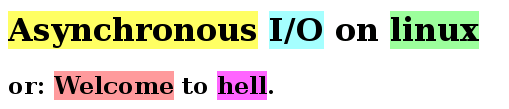
\includegraphics[width=.7\textwidth]{images/aio-linux.png}}\\
{\scriptsize (mirrored at \url{compgeom.com/~piyush/teach/4531_06/project/hell.html})}
   \\[3em]

   ``Asynchronous I/O, for example, is often infuriating.''\\
--- Robert Love. {\em Linux System Programming, 2nd ed, } page 215.
  

\end{frame}
%%%%%%%%%%%%%%%%%%%%%%%%%%%%%%%%%%%%%%%%%%%%%%%%%%%%%%%%%%%%%%%%%%%%%%%%%%%%%%%%

%%%%%%%%%%%%%%%%%%%%%%%%%%%%%%%%%%%%%%%%%%%%%%%%%%%%%%%%%%%%%%%%%%%%%%%%%%%%%%%%
\begin{frame}[fragile]
  \frametitle{Why non-blocking I/O?}
  
  Consider some I/O:


\begin{minipage}{.5\textwidth}
\begin{lstlisting}
    fd = open(...);
    read(...);
    close(fd);
  \end{lstlisting}
\end{minipage}


  Not very performant---under what conditions do we lose out?

\end{frame}
%%%%%%%%%%%%%%%%%%%%%%%%%%%%%%%%%%%%%%%%%%%%%%%%%%%%%%%%%%%%%%%%%%%%%%%%%%%%%%%%

%%%%%%%%%%%%%%%%%%%%%%%%%%%%%%%%%%%%%%%%%%%%%%%%%%%%%%%%%%%%%%%%%%%%%%%%%%%%%%%%
\begin{frame}[fragile]
  \frametitle{Mitigating I/O impact}

    So far: can use threads to mitigate latency.\\

    What are the disadvantages?
    \only<2>{
      \begin{itemize}
        \item race conditions
        \item overhead/max \# of thread limitations
      \end{itemize}
    }

\end{frame}
%%%%%%%%%%%%%%%%%%%%%%%%%%%%%%%%%%%%%%%%%%%%%%%%%%%%%%%%%%%%%%%%%%%%%%%%%%%%%%%%


%%%%%%%%%%%%%%%%%%%%%%%%%%%%%%%%%%%%%%%%%%%%%%%%%%%%%%%%%%%%%%%%%%%%%%%%%%%%%%%%
\begin{frame}[fragile]
  \frametitle{An Alternative to Threads}

    Asynchronous/nonblocking I/O.\\[2em]


\begin{minipage}{.6\textwidth}
\begin{lstlisting}
    fd = open(..., O_NONBLOCK);
    read(...); // returns instantly!
    close(fd);
  \end{lstlisting}
\end{minipage}


\begin{center}
~\\[1em]
$\cdots$\\[2em]


\includegraphics[width=.25\textwidth]{images/Easy_button.JPG}
\end{center}
\hfill {\scriptsize (credit: Yskyflyer, Wikimedia Commons)}


\end{frame}
%%%%%%%%%%%%%%%%%%%%%%%%%%%%%%%%%%%%%%%%%%%%%%%%%%%%%%%%%%%%%%%%%%%%%%%%%%%%%%%%

%%%%%%%%%%%%%%%%%%%%%%%%%%%%%%%%%%%%%%%%%%%%%%%%%%%%%%%%%%%%%%%%%%%%%%%%%%%%%%%%
\begin{frame}
  \frametitle{Not Quite So Easy}

    Doesn't work on files---they're always ready. Only e.g. sockets.

\end{frame}
%%%%%%%%%%%%%%%%%%%%%%%%%%%%%%%%%%%%%%%%%%%%%%%%%%%%%%%%%%%%%%%%%%%%%%%%%%%%%%%%

%%%%%%%%%%%%%%%%%%%%%%%%%%%%%%%%%%%%%%%%%%%%%%%%%%%%%%%%%%%%%%%%%%%%%%%%%%%%%%%%
\begin{frame}
  \frametitle{Other Outstanding Problem with Nonblocking I/O}

    How do you know when I/O is ready to be queried?

    \only<2>{\begin{itemize} 
      \item polling ({\tt select}, {\tt poll}, {\tt epoll})
      \item interrupts (signals)
      \end{itemize}
    }

\end{frame}
%%%%%%%%%%%%%%%%%%%%%%%%%%%%%%%%%%%%%%%%%%%%%%%%%%%%%%%%%%%%%%%%%%%%%%%%%%%%%%%%

%%%%%%%%%%%%%%%%%%%%%%%%%%%%%%%%%%%%%%%%%%%%%%%%%%%%%%%%%%%%%%%%%%%%%%%%%%%%%%%%
\begin{frame}
  \frametitle{Using {\tt epoll}}
  
    Key idea: give {\tt epoll} a bunch of file descriptors;\\
     \hspace*{2em}wait for events to happen.\\[1em]

\begin{center}
	
\includegraphics[width=0.2\textwidth]{images/waitforit.jpg}
\end{center}

     Steps:
     \begin{enumerate}
       \item create an instance ({\tt epoll\_create1});
       \item populate it with file descriptors ({\tt epoll\_ctl});
       \item wait for events ({\tt epoll\_wait}).
     \end{enumerate}
  
\end{frame}
%%%%%%%%%%%%%%%%%%%%%%%%%%%%%%%%%%%%%%%%%%%%%%%%%%%%%%%%%%%%%%%%%%%%%%%%%%%%%%%%

%%%%%%%%%%%%%%%%%%%%%%%%%%%%%%%%%%%%%%%%%%%%%%%%%%%%%%%%%%%%%%%%%%%%%%%%%%%%%%%%
\begin{frame}[fragile]
  \frametitle{Creating an {\tt epoll} instance}
  
    \begin{minipage}{.5\textwidth}
    \begin{lstlisting}
   int epfd = epoll_create1(0);
    \end{lstlisting}
    \end{minipage}

    {\tt efpd} doesn't represent any files; use it to talk to {\tt epoll}.\\[1em]

    0 represents the flags (only flag: {\tt EPOLL\_CLOEXEC}).
    
  
\end{frame}
%%%%%%%%%%%%%%%%%%%%%%%%%%%%%%%%%%%%%%%%%%%%%%%%%%%%%%%%%%%%%%%%%%%%%%%%%%%%%%%%

%%%%%%%%%%%%%%%%%%%%%%%%%%%%%%%%%%%%%%%%%%%%%%%%%%%%%%%%%%%%%%%%%%%%%%%%%%%%%%%%
\begin{frame}[fragile]
  \frametitle{Populating the {\tt epoll} instance}
  
    To add {\tt fd} to the set of descriptors watched by {\tt epfd}:
    \begin{lstlisting}
   struct epoll_event event;
   int ret;
   event.data.fd = fd;
   event.events = EPOLLIN | EPOLLOUT;
   ret = epoll_ctl(epfd, EPOLL_CTL_ADD, fd, &event);
    \end{lstlisting}

    Can also modify and delete descriptors from {\tt epfd}.
  
\end{frame}
%%%%%%%%%%%%%%%%%%%%%%%%%%%%%%%%%%%%%%%%%%%%%%%%%%%%%%%%%%%%%%%%%%%%%%%%%%%%%%%%

%%%%%%%%%%%%%%%%%%%%%%%%%%%%%%%%%%%%%%%%%%%%%%%%%%%%%%%%%%%%%%%%%%%%%%%%%%%%%%%%
\begin{frame}[fragile]
  \frametitle{Waiting on an {\tt epoll} instance}
  
    Now we're ready to wait for events on any file descriptor in {\tt epfd}.
    \begin{lstlisting}
  #define MAX_EVENTS 64

  struct epoll_event events[MAX_EVENTS];
  int nr_events;

  nr_events = epoll_wait(epfd, events, MAX_EVENTS, -1);
    \end{lstlisting}

-1: wait potentially forever; otherwise, milliseconds to wait.\\[1em]

Upon return from {\tt epoll\_wait}, we have {\tt nr\_events} events ready.

  
\end{frame}
%%%%%%%%%%%%%%%%%%%%%%%%%%%%%%%%%%%%%%%%%%%%%%%%%%%%%%%%%%%%%%%%%%%%%%%%%%%%%%%%

%%%%%%%%%%%%%%%%%%%%%%%%%%%%%%%%%%%%%%%%%%%%%%%%%%%%%%%%%%%%%%%%%%%%%%%%%%%%%%%%


\begin{frame}[fragile]
\frametitle{epoll Example}

\begin{lstlisting}[language=C]
#define MAX_EVENTS 10
struct epoll_event ev, events[MAX_EVENTS];
int listen_sock, conn_sock, nfds, epollfd;

/* Code to set up listening socket, 'listen_sock',
   (socket(), bind(), listen()) omitted */

epollfd = epoll_create1(0);
if (epollfd == -1) {
    perror("epoll_create1");
    exit(EXIT_FAILURE);
}

ev.events = EPOLLIN;
ev.data.fd = listen_sock;
if (epoll_ctl(epollfd, EPOLL_CTL_ADD, listen_sock, &ev) == -1) {
    perror("epoll_ctl: listen_sock");
    exit(EXIT_FAILURE);
}
\end{lstlisting}


\end{frame}

\begin{frame}[fragile]
\frametitle{epoll Example}

\begin{lstlisting}[language=C]
for (;;) {
    nfds = epoll_wait(epollfd, events, MAX_EVENTS, -1);
    if (nfds == -1) {
        perror("epoll_wait");
        exit(EXIT_FAILURE);
    }

    for (n = 0; n < nfds; ++n) {
        if (events[n].data.fd == listen_sock) {
            conn_sock = accept(listen_sock, (struct sockaddr *) &addr, &addrlen);
            if (conn_sock == -1) {
                perror("accept");
                exit(EXIT_FAILURE);
            }
            setnonblocking(conn_sock);
            ev.events = EPOLLIN | EPOLLET;
            ev.data.fd = conn_sock;
            if (epoll_ctl(epollfd, EPOLL_CTL_ADD, conn_sock,
                        &ev) == -1) {
                perror("epoll_ctl: conn_sock");
                exit(EXIT_FAILURE);
            }
        } else {
            do_use_fd(events[n].data.fd);
        }
    }
}
\end{lstlisting}


\end{frame}


%%%%%%%%%%%%%%%%%%%%%%%%%%%%%%%%%%%%%%%%%%%%%%%%%%%%%%%%%%%%%%%%%%%%%%%%%%%%%%%%
\begin{frame}
  \frametitle{Nonblocking I/O with curl}
  
    Similar idea to {\tt epoll}:
\begin{itemize}
\item build up a set of descriptors;
\item invoke the transfers and wait for them to finish;
\item see how things went.
\end{itemize}
  
\end{frame}
%%%%%%%%%%%%%%%%%%%%%%%%%%%%%%%%%%%%%%%%%%%%%%%%%%%%%%%%%%%%%%%%%%%%%%%%%%%%%%%%


\begin{frame}[fragile]
\frametitle{Classic, Blocking cURL Request}

Here's a simple cURL program that we can look over:

\begin{lstlisting}[language=C]
#include <stdio.h>
#include <curl/curl.h>
 
int main( int argc, char** argv ) {
  CURL *curl;
  CURLcode res;
 
  curl_global_init(CURL_GLOBAL_DEFAULT);
 
  curl = curl_easy_init();
  if( curl ) {
    curl_easy_setopt(curl, CURLOPT_URL, "https://example.com/" );
    res = curl_easy_perform( curl );
    
  if( res != CURLE_OK ) {
      fprintf(stderr, "curl_easy_perform() failed: %s\n", curl_easy_strerror(res));
    }
    curl_easy_cleanup(curl);
  }
 
  curl_global_cleanup();
  return 0;
}
\end{lstlisting}


\end{frame}



%%%%%%%%%%%%%%%%%%%%%%%%%%%%%%%%%%%%%%%%%%%%%%%%%%%%%%%%%%%%%%%%%%%%%%%%%%%%%%%%
\begin{frame}
  \frametitle{curl\_multi initialization}

  
    curl\_multi: work with multiple resources at once.\\[1em]
    
    1. To use {\tt curl\_multi}, first create the individual requests \\ \hspace{2em} ({\tt curl\_easy\_init}).\\
    ~~~(Set options as needed on each handle).\\[1em]

    2. Then, combine them with:
    \begin{itemize}
      \item {\tt curl\_multi\_init()};
      \item {\tt curl\_multi\_add\_handle()}.
    \end{itemize}

  

\end{frame}
%%%%%%%%%%%%%%%%%%%%%%%%%%%%%%%%%%%%%%%%%%%%%%%%%%%%%%%%%%%%%%%%%%%%%%%%%%%%%%%%


\begin{frame}
\frametitle{Open Fire!}

Start reqs: \texttt{curl\_multi\_perform( CURLM* cm, int* still\_running )}

\begin{center}
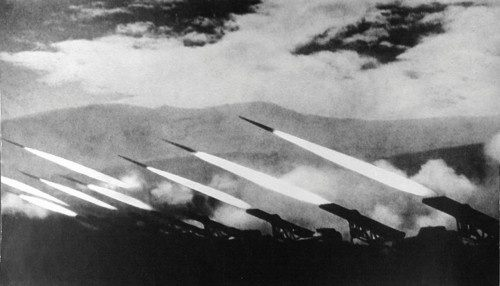
\includegraphics[width=0.5\textwidth]{images/artillery.jpeg}
\end{center}

The second parameter is updated with the number of still-in-progress requests.

Meantime, we can do other things!

\end{frame}


\begin{frame}[fragile]
\frametitle{I'm bored... So take a nap?}

Suppose we've run out of things to do and nothing is ready yet. Wait!

\begin{lstlisting}[language=C]
curl_multi_wait( CURLM *multi_handle, struct curl_waitfd extra_fds[], 
unsigned int extra_nfds, int timeout_ms, int *numfds )
\end{lstlisting}

This function will block the current thread until something happens.

Choose how long to wait and see how many events occurred.

\end{frame}


\begin{frame}
\frametitle{While You Were Sleeping}

While we are asleep or doing other things, callbacks still happen.

The status of the cURL easy handle is updated.

\end{frame}




%%%%%%%%%%%%%%%%%%%%%%%%%%%%%%%%%%%%%%%%%%%%%%%%%%%%%%%%%%%%%%%%%%%%%%%%%%%%%%%%
\begin{frame}[fragile]
  \frametitle{Knowing what happened after {\tt curl\_multi\_perform}}

  
    {\tt curl\_multi\_info\_read} will tell you.
  
\begin{lstlisting}
  msg = curl_multi_info_read(multi_handle, &msgs_left);
\end{lstlisting}
  
    and also how many messages are left.\\[1em]
    {\tt msg->msg} can be {\tt CURLMSG\_DONE} or an error;\\
    {\tt msg->easy\_handle} tells you who is done.\\[1em]
  

    Some gotchas (thanks Desiye Collier):
    \begin{itemize}
    \item Checking \verb+msg->msg == CURLMSG_DONE+ is not sufficient to ensure that a curl request actually happened. You also need to check {\tt data.result}.

    \item (A1 hint:) To reset an individual handle in the {\tt multi\_handle}, you need to ``replace'' it. But you shouldn't use {\tt curl\_easy\_init()}.  In fact, you don't need a new handle at all.
    \end{itemize}
  

\end{frame}
%%%%%%%%%%%%%%%%%%%%%%%%%%%%%%%%%%%%%%%%%%%%%%%%%%%%%%%%%%%%%%%%%%%%%%%%%%%%%%%%



%%%%%%%%%%%%%%%%%%%%%%%%%%%%%%%%%%%%%%%%%%%%%%%%%%%%%%%%%%%%%%%%%%%%%%%%%%%%%%%%
\begin{frame}
  \frametitle{curl\_multi cleanup}

  
    Call {\tt curl\_multi\_cleanup} on the multi handle.\\[1em]
    Then, call {\tt curl\_easy\_cleanup} on each easy handle.\\[2em]
    If you replace {\tt curl\_easy\_init} by {\tt curl\_global\_init},\\
    then call {\tt curl\_global\_cleanup} also.
  

\end{frame}
%%%%%%%%%%%%%%%%%%%%%%%%%%%%%%%%%%%%%%%%%%%%%%%%%%%%%%%%%%%%%%%%%%%%%%%%%%%%%%%%

\begin{frame}[fragile]
	\frametitle{cURL Multi Example}

	\begin{lstlisting}[language=C]
#include <stdio.h>
#include <stdlib.h>
#include <unistd.h>
#include <curl/multi.h>

#define MAX_WAIT_MSECS 30*1000 /* Wait max. 30 seconds */

const char *urls[] = {
  "http://www.microsoft.com",
  "http://www.yahoo.com",
  "http://www.wikipedia.org",
  "http://slashdot.org"
};
#define CNT 4

size_t cb(char *d, size_t n, size_t l, void *p) {
  /* take care of the data here, ignored in this example */
  return n*l;
\end{lstlisting}

\end{frame}

\begin{frame}[fragile]
	\frametitle{cURL Multi Example}

	\begin{lstlisting}[language=C]
void init( CURLM *cm, int i ) {
  CURL *eh = curl_easy_init();
  curl_easy_setopt( eh, CURLOPT_WRITEFUNCTION, cb );
  curl_easy_setopt( eh, CURLOPT_HEADER, 0L );
  curl_easy_setopt( eh, CURLOPT_URL, urls[i] );
  curl_easy_setopt( eh, CURLOPT_PRIVATE, urls[i]) ;
  curl_easy_setopt( eh, CURLOPT_VERBOSE, 0L );
  curl_multi_add_handle( cm, eh );
}

int main( int argc, char** argv ) {
    CURLM *cm = NULL;
    CURL *eh = NULL;
    CURLMsg *msg = NULL;
    CURLcode return_code = 0;
    int still_running = 0; 
    int msgs_left = 0;
    int http_status_code;
    const char *szUrl;

    curl_global_init( CURL_GLOBAL_ALL );
    cm = curl_multi_init( );
    
    for ( int i = 0; i < CNT; ++i ) {
        init( cm, i );
    }
\end{lstlisting}

\end{frame}

\begin{frame}[fragile]
	\frametitle{cURL Multi Example}

	\begin{lstlisting}[language=C]
    curl_multi_perform( cm, &still_running );

    do {
        int numfds = 0;
        int res = curl_multi_wait( cm, NULL, 0, MAX_WAIT_MSECS, &numfds );
        if( res != CURLM_OK ) {
            fprintf( stderr, "error: curl_multi_wait() returned %d\n", res );
            return EXIT_FAILURE;
        }
        curl_multi_perform( cm, &still_running );

    } while( still_running );
\end{lstlisting}

\end{frame}

\begin{frame}[fragile]
	\frametitle{cURL Multi Example}

	\begin{lstlisting}[language=C]
    while ( ( msg = curl_multi_info_read( cm, &msgs_left ) ) ) {
        if ( msg->msg == CURLMSG_DONE ) {
            eh = msg->easy_handle;
            return_code = msg->data.result;
            if ( return_code != CURLE_OK ) {
                fprintf( stderr, "CURL error code: %d\n", msg->data.result );
                curl_multi_remove_handle( cm, eh );
                curl_easy_cleanup( eh );
                continue;
            }
            http_status_code = 0; szUrl = NULL;
            curl_easy_getinfo( eh, CURLINFO_RESPONSE_CODE, &http_status_code );
            curl_easy_getinfo( eh, CURLINFO_PRIVATE, &szUrl );

            if( http_status_code == 200 ) {
                printf( "200 OK for %s\n", szUrl ) ;
            } else {
                fprintf( stderr, "GET of %s returned http status code %d\n",
                     szUrl, http_status_code );
            }
            curl_multi_remove_handle( cm, eh );
            curl_easy_cleanup( eh );
        } else {
            fprintf( stderr, "error: after curl_multi_info_read(), CURLMsg=%d\n", msg->msg );
        }
    }
\end{lstlisting}

\end{frame}

\begin{frame}[fragile]
	\frametitle{cURL Multi Example}

	\begin{lstlisting}[language=C]
    curl_multi_cleanup( cm );
    curl_global_cleanup();
    return 0;
}
\end{lstlisting}

\end{frame}


\begin{frame}
	\frametitle{Scaling This}

	The developer claims that you can have multiple thousands of connections in a single multi handle.

	60k ought to be enough for anyone!
\end{frame}


\begin{frame}
	\frametitle{cURL + select}
	\begin{center}
		
\includegraphics[width=0.55\textwidth]{images/harold.jpg}
	\end{center}


\end{frame}


%%%%%%%%%%%%%%%%%%%%%%%%%%%%%%%%%%%%%%%%%%%%%%%%%%%%%%%%%%%%%%%%%%%%%%%%%%%%%%%%
\begin{frame}
  \frametitle{Process, Threads, AIO?! Four Choices}

  
    \begin{itemize}
      \item Blocking I/O; 1 process per request.
      \item Blocking I/O; 1 thread per request.
      \item Asynchronous I/O, pool of threads, \\callbacks, \\ each thread handles multiple connections.
      \item Nonblocking I/O, pool of threads, \\ multiplexed with select/poll,
        event-driven, \\ each thread handles multiple connections.
    \end{itemize}
  

\end{frame}
%%%%%%%%%%%%%%%%%%%%%%%%%%%%%%%%%%%%%%%%%%%%%%%%%%%%%%%%%%%%%%%%%%%%%%%%%%%%%%%%

%%%%%%%%%%%%%%%%%%%%%%%%%%%%%%%%%%%%%%%%%%%%%%%%%%%%%%%%%%%%%%%%%%%%%%%%%%%%%%%%
\begin{frame}
  \frametitle{Blocking I/O; 1 process per request}

  
  Old Apache model: \hfill 
\includegraphics[width=.2\textwidth]{images/httpd_logo_wide_new}

  \begin{itemize}
    \item Main thread waits for connections.
    \item Upon connect, forks off a new process, \\which completely
      handles the connection.
    \item Each I/O request is blocking: \\ e.g. reads wait until more data arrives.
  \end{itemize}

  Advantage: 
  \begin{itemize}
    \item ``Simple to understand and easy to program.''
  \end{itemize}

  Disadvantage:
  \begin{itemize}
    \item High overhead from starting 1000s of processes.\\
      (can somewhat mitigate with process pool).
  \end{itemize}
  Can handle $\sim$10 000 processes, but doesn't generally scale.

  

\end{frame}
%%%%%%%%%%%%%%%%%%%%%%%%%%%%%%%%%%%%%%%%%%%%%%%%%%%%%%%%%%%%%%%%%%%%%%%%%%%%%%%%

%%%%%%%%%%%%%%%%%%%%%%%%%%%%%%%%%%%%%%%%%%%%%%%%%%%%%%%%%%%%%%%%%%%%%%%%%%%%%%%%
\begin{frame}
  \frametitle{Blocking I/O; 1 thread per request}

  
    We know that threads are more lightweight than processes.\\[1em]

    Same as 1 process per request, but less overhead.\\[1em]

    I/O is the same---still blocking.\\[1em]

    Advantage:
    \begin{itemize}
      \item Still simple to understand and easy to program.
    \end{itemize}

    Disadvantages:
    \begin{itemize}
      \item Overhead still piles up, although less than processes.
      \item New complication: race conditions on shared data.
    \end{itemize}
  
\end{frame}
%%%%%%%%%%%%%%%%%%%%%%%%%%%%%%%%%%%%%%%%%%%%%%%%%%%%%%%%%%%%%%%%%%%%%%%%%%%%%%%%

%%%%%%%%%%%%%%%%%%%%%%%%%%%%%%%%%%%%%%%%%%%%%%%%%%%%%%%%%%%%%%%%%%%%%%%%%%%%%%%%
\begin{frame}
  \frametitle{Asynchronous I/O Benefits}

  
    In 2006, perf benefits of asynchronous I/O on lighttpd\footnote{\tiny \url{http://blog.lighttpd.net/articles/2006/11/12/lighty-1-5-0-and-linux-aio/}}:\\

{\small
    \begin{tabular}{llrrr}
    version & & fetches/sec & bytes/sec & CPU idle \\
    1.4.13 & sendfile & 36.45 & 3.73e+06 & 16.43\% \\
    1.5.0 & sendfile & 40.51 & 4.14e+06 & 12.77\% \\
    1.5.0 & linux-aio-sendfile & 72.70 & 7.44e+06 & 46.11\% \\
    \end{tabular}
}~\\[1em]

    (Workload: $2\times 7200$ RPM in RAID1, 1GB RAM, \\
     \qquad transferring 10GBytes on a 100MBit network).\\[1em]
  
\end{frame}
%%%%%%%%%%%%%%%%%%%%%%%%%%%%%%%%%%%%%%%%%%%%%%%%%%%%%%%%%%%%%%%%%%%%%%%%%%%%%%%%

%%%%%%%%%%%%%%%%%%%%%%%%%%%%%%%%%%%%%%%%%%%%%%%%%%%%%%%%%%%%%%%%%%%%%%%%%%%%%%%%
\begin{frame}
  \frametitle{Using Asynchronous I/O in Linux (select/poll)}


   Basic workflow: \\[1em]
   \begin{enumerate}
     \item enqueue a request;
     \item \ldots ~do something else;
     \item (if needed) periodically check whether request is done; and
     \item read the return value.
   \end{enumerate}

  
\end{frame}
%%%%%%%%%%%%%%%%%%%%%%%%%%%%%%%%%%%%%%%%%%%%%%%%%%%%%%%%%%%%%%%%%%%%%%%%%%%%%%%%


\end{document}

